
% !TeX document-id = {d8b4925c-2057-42a4-b894-2f1a3f1b6345}
%!TeX TXS-program:compile = txs:///xelatex/[--shell-escape]
\documentclass[aspectratio=169, mathserif]{beamer}% TPU recommends 16:9 ratio, 4:3 may require some work with inner theme .sty file

% Style options:
% light --- light theme (default)
% dark --- dark theme
% enlogo --- english TPU logo {default}
% rulogo --- russian TPU logo

\usetheme[light, rulogo]{tpu}% dark theme used as an example of optional argument

\usepackage[russian]{babel}%uncomment this to work in russian
\usepackage[utf8]{inputenc}

\usepackage{fontspec}

\setromanfont{Brygada1918}[
Path=./fonts/BrygadaFontFiles/,
Extension = .ttf,
UprightFont=*-Regular,
BoldFont=*-Bold,
ItalicFont=*-Italic,
BoldItalicFont=*-BoldItalic
]

\setsansfont{ALSSirius}[
Path=./fonts/ALSSiriusFiles/,
Extension = .otf,
UprightFont=*-Regular,
BoldFont=*-Bold,
%ItalicFont=*-Italic,
%BoldItalicFont=*-BoldItalic
]

\setmonofont{Consolas}[
Path=./fonts/ConsolasFontFiles/,
%Scale=0.85,
Extension = .ttf,
UprightFont=*-Regular,
BoldFont=*-Bold,
ItalicFont=*-Italic,
BoldItalicFont=*-BoldItalic
]

\usepackage[cache=false]{minted}
\usepackage{xcolor} % to access the named colour LightGray
\definecolor{LightGray}{gray}{0.9}
\definecolor{onedarkBckGr}{RGB}{40, 44, 52}

\usemintedstyle[python]{default}
\setminted[python]{
fontsize=\scriptsize,
escapeinside=||,
mathescape=true,
numbersep=5pt,
gobble=2,
linenos=true,
frame=leftline,
framesep=1mm,
python3=true,
%bgcolor=backcolour,
}

\usemintedstyle[pycon]{default}
\setminted[pycon]{
	fontsize=\scriptsize,
	escapeinside=||,
	mathescape=true,
	numbersep=5pt,
	gobble=2,
	frame=single,
	framesep=1mm,
	python3=true,
%	bgcolor=backcolour,
	linenos=true,
}

\newmint{python}{}

\usepackage{booktabs}% good looking tables
\usepackage{multicol}% text in multiple columns, useful for side-by-side text and pictures
\usepackage{hyperref}
\definecolor{maroon}{cmyk}{0, 0.87, 0.68, 0.32}
\definecolor{halfgray}{gray}{0.55}
\definecolor{ipython_frame}{RGB}{207, 207, 207}
\definecolor{ipython_bg}{RGB}{247, 247, 247}
\definecolor{ipython_red}{RGB}{186, 33, 33}
\definecolor{ipython_green}{RGB}{0, 128, 0}
\definecolor{ipython_cyan}{RGB}{64, 128, 128}
\definecolor{ipython_purple}{RGB}{170, 34, 255}
\definecolor{linkcolor}{HTML}{0000FF} % цвет гиперссылок
\definecolor{urlcolor}{HTML}{800080} % цвет ссылок
\definecolor{backcolour}{rgb}{0.95,0.95,0.92}

\usepackage{longtable}
\usepackage{wrapfig}
\usepackage{ragged2e}
\usepackage[nooneline]{caption}
\DeclareCaptionTextFormat{center}{\centering{#1}}
\captionsetup[table]{justification=raggedleft,
labelformat=empty,
labelsep=endash,
textformat=center,
position=top,
skip=5pt
}

\hyphenpenalty=10000% i don’t think hyphenation in presentations is a good idea, feel free to change however you like

\usepackage{chemfig}

%\usepackage[breakable]{tcolorbox}
%    \usepackage{parskip} % Stop auto-indenting (to mimic markdown behaviour)

    \usepackage{iftex}
    \ifPDFTeX
        \usepackage[T1]{fontenc}
        \usepackage{mathpazo}
    \else
        \usepackage{fontspec}
    \fi

    % Basic figure setup, for now with no caption control since it's done
    % automatically by Pandoc (which extracts ![](path) syntax from Markdown).
%    \usepackage{graphicx}
    % Maintain compatibility with old templates. Remove in nbconvert 6.0
    \let\Oldincludegraphics\includegraphics
    % Ensure that by default, figures have no caption (until we provide a
    % proper Figure object with a Caption API and a way to capture that
    % in the conversion process - todo).
    \usepackage{caption}
    \DeclareCaptionFormat{nocaption}{}
    \captionsetup{format=nocaption,aboveskip=0pt,belowskip=0pt}

    \usepackage[Export]{adjustbox} % Used to constrain images to a maximum size
    \adjustboxset{max size={0.9\linewidth}{0.9\paperheight}}
    \usepackage{float}
    \floatplacement{figure}{H} % forces figures to be placed at the correct location
%    \usepackage{xcolor} % Allow colors to be defined
%    \usepackage{enumerate} % Needed for markdown enumerations to work
%    \usepackage{geometry} % Used to adjust the document margins
%    \usepackage{amsmath} % Equations
%    \usepackage{amssymb} % Equations
    \usepackage{textcomp} % defines textquotesingle
    % Hack from http://tex.stackexchange.com/a/47451/13684:
    \AtBeginDocument{%
        \def\PYZsq{\textquotesingle}% Upright quotes in Pygmentized code
    }
    \usepackage{upquote} % Upright quotes for verbatim code
    \usepackage{eurosym} % defines \euro
    \usepackage[mathletters]{ucs} % Extended unicode (utf-8) support
    \usepackage{fancyvrb} % verbatim replacement that allows latex
    \usepackage{grffile} % extends the file name processing of package graphics
                         % to support a larger range
    \makeatletter % fix for grffile with XeLaTeX
    \def\Gread@@xetex#1{%
      \IfFileExists{"\Gin@base".bb}%
      {\Gread@eps{\Gin@base.bb}}%
      {\Gread@@xetex@aux#1}%
    }
    \makeatother

    % The hyperref package gives us a pdf with properly built
    % internal navigation ('pdf bookmarks' for the table of contents,
    % internal cross-reference links, web links for URLs, etc.)
%    \usepackage{hyperref}
    % The default LaTeX title has an obnoxious amount of whitespace. By default,
    % titling removes some of it. It also provides customization options.
%    \usepackage{titling}
    \usepackage{longtable} % longtable support required by pandoc >1.10
    \usepackage{booktabs}  % table support for pandoc > 1.12.2
%    \usepackage[inline]{enumitem} % IRkernel/repr support (it uses the enumerate* environment)
    \usepackage[normalem]{ulem} % ulem is needed to support strikethroughs (\sout)
                                % normalem makes italics be italics, not underlines
    \usepackage{mathrsfs}



    % Colors for the hyperref package
    \definecolor{urlcolor}{rgb}{0,.145,.698}
    \definecolor{linkcolor}{rgb}{.71,0.21,0.01}
    \definecolor{citecolor}{rgb}{.12,.54,.11}

    % ANSI colors
    \definecolor{ansi-black}{HTML}{3E424D}
    \definecolor{ansi-black-intense}{HTML}{282C36}
    \definecolor{ansi-red}{HTML}{E75C58}
    \definecolor{ansi-red-intense}{HTML}{B22B31}
    \definecolor{ansi-green}{HTML}{00A250}
    \definecolor{ansi-green-intense}{HTML}{007427}
    \definecolor{ansi-yellow}{HTML}{DDB62B}
    \definecolor{ansi-yellow-intense}{HTML}{B27D12}
    \definecolor{ansi-blue}{HTML}{208FFB}
    \definecolor{ansi-blue-intense}{HTML}{0065CA}
    \definecolor{ansi-magenta}{HTML}{D160C4}
    \definecolor{ansi-magenta-intense}{HTML}{A03196}
    \definecolor{ansi-cyan}{HTML}{60C6C8}
    \definecolor{ansi-cyan-intense}{HTML}{258F8F}
    \definecolor{ansi-white}{HTML}{C5C1B4}
    \definecolor{ansi-white-intense}{HTML}{A1A6B2}
    \definecolor{ansi-default-inverse-fg}{HTML}{FFFFFF}
    \definecolor{ansi-default-inverse-bg}{HTML}{000000}

    % commands and environments needed by pandoc snippets
    % extracted from the output of `pandoc -s`
    \providecommand{\tightlist}{%
      \setlength{\itemsep}{0pt}\setlength{\parskip}{0pt}}
    \DefineVerbatimEnvironment{Highlighting}{Verbatim}{commandchars=\\\{\}}
    % Add ',fontsize=\small' for more characters per line
    \newenvironment{Shaded}{}{}
    \newcommand{\KeywordTok}[1]{\textcolor[rgb]{0.00,0.44,0.13}{\textbf{{#1}}}}
    \newcommand{\DataTypeTok}[1]{\textcolor[rgb]{0.56,0.13,0.00}{{#1}}}
    \newcommand{\DecValTok}[1]{\textcolor[rgb]{0.25,0.63,0.44}{{#1}}}
    \newcommand{\BaseNTok}[1]{\textcolor[rgb]{0.25,0.63,0.44}{{#1}}}
    \newcommand{\FloatTok}[1]{\textcolor[rgb]{0.25,0.63,0.44}{{#1}}}
    \newcommand{\CharTok}[1]{\textcolor[rgb]{0.25,0.44,0.63}{{#1}}}
    \newcommand{\StringTok}[1]{\textcolor[rgb]{0.25,0.44,0.63}{{#1}}}
    \newcommand{\CommentTok}[1]{\textcolor[rgb]{0.38,0.63,0.69}{\textit{{#1}}}}
    \newcommand{\OtherTok}[1]{\textcolor[rgb]{0.00,0.44,0.13}{{#1}}}
    \newcommand{\AlertTok}[1]{\textcolor[rgb]{1.00,0.00,0.00}{\textbf{{#1}}}}
    \newcommand{\FunctionTok}[1]{\textcolor[rgb]{0.02,0.16,0.49}{{#1}}}
    \newcommand{\RegionMarkerTok}[1]{{#1}}
    \newcommand{\ErrorTok}[1]{\textcolor[rgb]{1.00,0.00,0.00}{\textbf{{#1}}}}
    \newcommand{\NormalTok}[1]{{#1}}

    % Additional commands for more recent versions of Pandoc
    \newcommand{\ConstantTok}[1]{\textcolor[rgb]{0.53,0.00,0.00}{{#1}}}
    \newcommand{\SpecialCharTok}[1]{\textcolor[rgb]{0.25,0.44,0.63}{{#1}}}
    \newcommand{\VerbatimStringTok}[1]{\textcolor[rgb]{0.25,0.44,0.63}{{#1}}}
    \newcommand{\SpecialStringTok}[1]{\textcolor[rgb]{0.73,0.40,0.53}{{#1}}}
    \newcommand{\ImportTok}[1]{{#1}}
    \newcommand{\DocumentationTok}[1]{\textcolor[rgb]{0.73,0.13,0.13}{\textit{{#1}}}}
    \newcommand{\AnnotationTok}[1]{\textcolor[rgb]{0.38,0.63,0.69}{\textbf{\textit{{#1}}}}}
    \newcommand{\CommentVarTok}[1]{\textcolor[rgb]{0.38,0.63,0.69}{\textbf{\textit{{#1}}}}}
    \newcommand{\VariableTok}[1]{\textcolor[rgb]{0.10,0.09,0.49}{{#1}}}
    \newcommand{\ControlFlowTok}[1]{\textcolor[rgb]{0.00,0.44,0.13}{\textbf{{#1}}}}
    \newcommand{\OperatorTok}[1]{\textcolor[rgb]{0.40,0.40,0.40}{{#1}}}
    \newcommand{\BuiltInTok}[1]{{#1}}
    \newcommand{\ExtensionTok}[1]{{#1}}
    \newcommand{\PreprocessorTok}[1]{\textcolor[rgb]{0.74,0.48,0.00}{{#1}}}
    \newcommand{\AttributeTok}[1]{\textcolor[rgb]{0.49,0.56,0.16}{{#1}}}
    \newcommand{\InformationTok}[1]{\textcolor[rgb]{0.38,0.63,0.69}{\textbf{\textit{{#1}}}}}
    \newcommand{\WarningTok}[1]{\textcolor[rgb]{0.38,0.63,0.69}{\textbf{\textit{{#1}}}}}


    % Define a nice break command that doesn't care if a line doesn't already
    % exist.
    \def\br{\hspace*{\fill} \\* }
    % Math Jax compatibility definitions
    \def\gt{>}
    \def\lt{<}
    \let\Oldtex\TeX
    \let\Oldlatex\LaTeX
    \renewcommand{\TeX}{\textrm{\Oldtex}}
    \renewcommand{\LaTeX}{\textrm{\Oldlatex}}
    % Document parameters
    % Document title
    \title{Untitled8}

% Pygments definitions
\makeatletter
\def\PY@reset{\let\PY@it=\relax \let\PY@bf=\relax%
    \let\PY@ul=\relax \let\PY@tc=\relax%
    \let\PY@bc=\relax \let\PY@ff=\relax}
\def\PY@tok#1{\csname PY@tok@#1\endcsname}
\def\PY@toks#1+{\ifx\relax#1\empty\else%
    \PY@tok{#1}\expandafter\PY@toks\fi}
\def\PY@do#1{\PY@bc{\PY@tc{\PY@ul{%
    \PY@it{\PY@bf{\PY@ff{#1}}}}}}}
\def\PY#1#2{\PY@reset\PY@toks#1+\relax+\PY@do{#2}}

\expandafter\def\csname PY@tok@w\endcsname{\def\PY@tc##1{\textcolor[rgb]{0.73,0.73,0.73}{##1}}}
\expandafter\def\csname PY@tok@c\endcsname{\let\PY@it=\textit\def\PY@tc##1{\textcolor[rgb]{0.25,0.50,0.50}{##1}}}
\expandafter\def\csname PY@tok@cp\endcsname{\def\PY@tc##1{\textcolor[rgb]{0.74,0.48,0.00}{##1}}}
\expandafter\def\csname PY@tok@k\endcsname{\let\PY@bf=\textbf\def\PY@tc##1{\textcolor[rgb]{0.00,0.50,0.00}{##1}}}
\expandafter\def\csname PY@tok@kp\endcsname{\def\PY@tc##1{\textcolor[rgb]{0.00,0.50,0.00}{##1}}}
\expandafter\def\csname PY@tok@kt\endcsname{\def\PY@tc##1{\textcolor[rgb]{0.69,0.00,0.25}{##1}}}
\expandafter\def\csname PY@tok@o\endcsname{\def\PY@tc##1{\textcolor[rgb]{0.40,0.40,0.40}{##1}}}
\expandafter\def\csname PY@tok@ow\endcsname{\let\PY@bf=\textbf\def\PY@tc##1{\textcolor[rgb]{0.67,0.13,1.00}{##1}}}
\expandafter\def\csname PY@tok@nb\endcsname{\def\PY@tc##1{\textcolor[rgb]{0.00,0.50,0.00}{##1}}}
\expandafter\def\csname PY@tok@nf\endcsname{\def\PY@tc##1{\textcolor[rgb]{0.00,0.00,1.00}{##1}}}
\expandafter\def\csname PY@tok@nc\endcsname{\let\PY@bf=\textbf\def\PY@tc##1{\textcolor[rgb]{0.00,0.00,1.00}{##1}}}
\expandafter\def\csname PY@tok@nn\endcsname{\let\PY@bf=\textbf\def\PY@tc##1{\textcolor[rgb]{0.00,0.00,1.00}{##1}}}
\expandafter\def\csname PY@tok@ne\endcsname{\let\PY@bf=\textbf\def\PY@tc##1{\textcolor[rgb]{0.82,0.25,0.23}{##1}}}
\expandafter\def\csname PY@tok@nv\endcsname{\def\PY@tc##1{\textcolor[rgb]{0.10,0.09,0.49}{##1}}}
\expandafter\def\csname PY@tok@no\endcsname{\def\PY@tc##1{\textcolor[rgb]{0.53,0.00,0.00}{##1}}}
\expandafter\def\csname PY@tok@nl\endcsname{\def\PY@tc##1{\textcolor[rgb]{0.63,0.63,0.00}{##1}}}
\expandafter\def\csname PY@tok@ni\endcsname{\let\PY@bf=\textbf\def\PY@tc##1{\textcolor[rgb]{0.60,0.60,0.60}{##1}}}
\expandafter\def\csname PY@tok@na\endcsname{\def\PY@tc##1{\textcolor[rgb]{0.49,0.56,0.16}{##1}}}
\expandafter\def\csname PY@tok@nt\endcsname{\let\PY@bf=\textbf\def\PY@tc##1{\textcolor[rgb]{0.00,0.50,0.00}{##1}}}
\expandafter\def\csname PY@tok@nd\endcsname{\def\PY@tc##1{\textcolor[rgb]{0.67,0.13,1.00}{##1}}}
\expandafter\def\csname PY@tok@s\endcsname{\def\PY@tc##1{\textcolor[rgb]{0.73,0.13,0.13}{##1}}}
\expandafter\def\csname PY@tok@sd\endcsname{\let\PY@it=\textit\def\PY@tc##1{\textcolor[rgb]{0.73,0.13,0.13}{##1}}}
\expandafter\def\csname PY@tok@si\endcsname{\let\PY@bf=\textbf\def\PY@tc##1{\textcolor[rgb]{0.73,0.40,0.53}{##1}}}
\expandafter\def\csname PY@tok@se\endcsname{\let\PY@bf=\textbf\def\PY@tc##1{\textcolor[rgb]{0.73,0.40,0.13}{##1}}}
\expandafter\def\csname PY@tok@sr\endcsname{\def\PY@tc##1{\textcolor[rgb]{0.73,0.40,0.53}{##1}}}
\expandafter\def\csname PY@tok@ss\endcsname{\def\PY@tc##1{\textcolor[rgb]{0.10,0.09,0.49}{##1}}}
\expandafter\def\csname PY@tok@sx\endcsname{\def\PY@tc##1{\textcolor[rgb]{0.00,0.50,0.00}{##1}}}
\expandafter\def\csname PY@tok@m\endcsname{\def\PY@tc##1{\textcolor[rgb]{0.40,0.40,0.40}{##1}}}
\expandafter\def\csname PY@tok@gh\endcsname{\let\PY@bf=\textbf\def\PY@tc##1{\textcolor[rgb]{0.00,0.00,0.50}{##1}}}
\expandafter\def\csname PY@tok@gu\endcsname{\let\PY@bf=\textbf\def\PY@tc##1{\textcolor[rgb]{0.50,0.00,0.50}{##1}}}
\expandafter\def\csname PY@tok@gd\endcsname{\def\PY@tc##1{\textcolor[rgb]{0.63,0.00,0.00}{##1}}}
\expandafter\def\csname PY@tok@gi\endcsname{\def\PY@tc##1{\textcolor[rgb]{0.00,0.63,0.00}{##1}}}
\expandafter\def\csname PY@tok@gr\endcsname{\def\PY@tc##1{\textcolor[rgb]{1.00,0.00,0.00}{##1}}}
\expandafter\def\csname PY@tok@ge\endcsname{\let\PY@it=\textit}
\expandafter\def\csname PY@tok@gs\endcsname{\let\PY@bf=\textbf}
\expandafter\def\csname PY@tok@gp\endcsname{\let\PY@bf=\textbf\def\PY@tc##1{\textcolor[rgb]{0.00,0.00,0.50}{##1}}}
\expandafter\def\csname PY@tok@go\endcsname{\def\PY@tc##1{\textcolor[rgb]{0.53,0.53,0.53}{##1}}}
\expandafter\def\csname PY@tok@gt\endcsname{\def\PY@tc##1{\textcolor[rgb]{0.00,0.27,0.87}{##1}}}
\expandafter\def\csname PY@tok@err\endcsname{\def\PY@bc##1{\setlength{\fboxsep}{0pt}\fcolorbox[rgb]{1.00,0.00,0.00}{1,1,1}{\strut ##1}}}
\expandafter\def\csname PY@tok@kc\endcsname{\let\PY@bf=\textbf\def\PY@tc##1{\textcolor[rgb]{0.00,0.50,0.00}{##1}}}
\expandafter\def\csname PY@tok@kd\endcsname{\let\PY@bf=\textbf\def\PY@tc##1{\textcolor[rgb]{0.00,0.50,0.00}{##1}}}
\expandafter\def\csname PY@tok@kn\endcsname{\let\PY@bf=\textbf\def\PY@tc##1{\textcolor[rgb]{0.00,0.50,0.00}{##1}}}
\expandafter\def\csname PY@tok@kr\endcsname{\let\PY@bf=\textbf\def\PY@tc##1{\textcolor[rgb]{0.00,0.50,0.00}{##1}}}
\expandafter\def\csname PY@tok@bp\endcsname{\def\PY@tc##1{\textcolor[rgb]{0.00,0.50,0.00}{##1}}}
\expandafter\def\csname PY@tok@fm\endcsname{\def\PY@tc##1{\textcolor[rgb]{0.00,0.00,1.00}{##1}}}
\expandafter\def\csname PY@tok@vc\endcsname{\def\PY@tc##1{\textcolor[rgb]{0.10,0.09,0.49}{##1}}}
\expandafter\def\csname PY@tok@vg\endcsname{\def\PY@tc##1{\textcolor[rgb]{0.10,0.09,0.49}{##1}}}
\expandafter\def\csname PY@tok@vi\endcsname{\def\PY@tc##1{\textcolor[rgb]{0.10,0.09,0.49}{##1}}}
\expandafter\def\csname PY@tok@vm\endcsname{\def\PY@tc##1{\textcolor[rgb]{0.10,0.09,0.49}{##1}}}
\expandafter\def\csname PY@tok@sa\endcsname{\def\PY@tc##1{\textcolor[rgb]{0.73,0.13,0.13}{##1}}}
\expandafter\def\csname PY@tok@sb\endcsname{\def\PY@tc##1{\textcolor[rgb]{0.73,0.13,0.13}{##1}}}
\expandafter\def\csname PY@tok@sc\endcsname{\def\PY@tc##1{\textcolor[rgb]{0.73,0.13,0.13}{##1}}}
\expandafter\def\csname PY@tok@dl\endcsname{\def\PY@tc##1{\textcolor[rgb]{0.73,0.13,0.13}{##1}}}
\expandafter\def\csname PY@tok@s2\endcsname{\def\PY@tc##1{\textcolor[rgb]{0.73,0.13,0.13}{##1}}}
\expandafter\def\csname PY@tok@sh\endcsname{\def\PY@tc##1{\textcolor[rgb]{0.73,0.13,0.13}{##1}}}
\expandafter\def\csname PY@tok@s1\endcsname{\def\PY@tc##1{\textcolor[rgb]{0.73,0.13,0.13}{##1}}}
\expandafter\def\csname PY@tok@mb\endcsname{\def\PY@tc##1{\textcolor[rgb]{0.40,0.40,0.40}{##1}}}
\expandafter\def\csname PY@tok@mf\endcsname{\def\PY@tc##1{\textcolor[rgb]{0.40,0.40,0.40}{##1}}}
\expandafter\def\csname PY@tok@mh\endcsname{\def\PY@tc##1{\textcolor[rgb]{0.40,0.40,0.40}{##1}}}
\expandafter\def\csname PY@tok@mi\endcsname{\def\PY@tc##1{\textcolor[rgb]{0.40,0.40,0.40}{##1}}}
\expandafter\def\csname PY@tok@il\endcsname{\def\PY@tc##1{\textcolor[rgb]{0.40,0.40,0.40}{##1}}}
\expandafter\def\csname PY@tok@mo\endcsname{\def\PY@tc##1{\textcolor[rgb]{0.40,0.40,0.40}{##1}}}
\expandafter\def\csname PY@tok@ch\endcsname{\let\PY@it=\textit\def\PY@tc##1{\textcolor[rgb]{0.25,0.50,0.50}{##1}}}
\expandafter\def\csname PY@tok@cm\endcsname{\let\PY@it=\textit\def\PY@tc##1{\textcolor[rgb]{0.25,0.50,0.50}{##1}}}
\expandafter\def\csname PY@tok@cpf\endcsname{\let\PY@it=\textit\def\PY@tc##1{\textcolor[rgb]{0.25,0.50,0.50}{##1}}}
\expandafter\def\csname PY@tok@c1\endcsname{\let\PY@it=\textit\def\PY@tc##1{\textcolor[rgb]{0.25,0.50,0.50}{##1}}}
\expandafter\def\csname PY@tok@cs\endcsname{\let\PY@it=\textit\def\PY@tc##1{\textcolor[rgb]{0.25,0.50,0.50}{##1}}}

\def\PYZbs{\char`\\}
\def\PYZus{\char`\_}
\def\PYZob{\char`\{}
\def\PYZcb{\char`\}}
\def\PYZca{\char`\^}
\def\PYZam{\char`\&}
\def\PYZlt{\char`\<}
\def\PYZgt{\char`\>}
\def\PYZsh{\char`\#}
\def\PYZpc{\char`\%}
\def\PYZdl{\char`\$}
\def\PYZhy{\char`\-}
\def\PYZsq{\char`\'}
\def\PYZdq{\char`\"}
\def\PYZti{\char`\~}
% for compatibility with earlier versions
\def\PYZat{@}
\def\PYZlb{[}
\def\PYZrb{]}
\makeatother


    % For linebreaks inside Verbatim environment from package fancyvrb.
    \makeatletter
        \newbox\Wrappedcontinuationbox
        \newbox\Wrappedvisiblespacebox
        \newcommand*\Wrappedvisiblespace {\textcolor{red}{\textvisiblespace}}
        \newcommand*\Wrappedcontinuationsymbol {\textcolor{red}{\llap{\tiny$\m@th\hookrightarrow$}}}
        \newcommand*\Wrappedcontinuationindent {3ex }
        \newcommand*\Wrappedafterbreak {\kern\Wrappedcontinuationindent\copy\Wrappedcontinuationbox}
        % Take advantage of the already applied Pygments mark-up to insert
        % potential linebreaks for TeX processing.
        %        {, <, #, %, $, ' and ": go to next line.
        %        _, }, ^, &, >, - and ~: stay at end of broken line.
        % Use of \textquotesingle for straight quote.
        \newcommand*\Wrappedbreaksatspecials {%
            \def\PYGZus{\discretionary{\char`\_}{\Wrappedafterbreak}{\char`\_}}%
            \def\PYGZob{\discretionary{}{\Wrappedafterbreak\char`\{}{\char`\{}}%
            \def\PYGZcb{\discretionary{\char`\}}{\Wrappedafterbreak}{\char`\}}}%
            \def\PYGZca{\discretionary{\char`\^}{\Wrappedafterbreak}{\char`\^}}%
            \def\PYGZam{\discretionary{\char`\&}{\Wrappedafterbreak}{\char`\&}}%
            \def\PYGZlt{\discretionary{}{\Wrappedafterbreak\char`\<}{\char`\<}}%
            \def\PYGZgt{\discretionary{\char`\>}{\Wrappedafterbreak}{\char`\>}}%
            \def\PYGZsh{\discretionary{}{\Wrappedafterbreak\char`\#}{\char`\#}}%
            \def\PYGZpc{\discretionary{}{\Wrappedafterbreak\char`\%}{\char`\%}}%
            \def\PYGZdl{\discretionary{}{\Wrappedafterbreak\char`\$}{\char`\$}}%
            \def\PYGZhy{\discretionary{\char`\-}{\Wrappedafterbreak}{\char`\-}}%
            \def\PYGZsq{\discretionary{}{\Wrappedafterbreak\textquotesingle}{\textquotesingle}}%
            \def\PYGZdq{\discretionary{}{\Wrappedafterbreak\char`\"}{\char`\"}}%
            \def\PYGZti{\discretionary{\char`\~}{\Wrappedafterbreak}{\char`\~}}%
        }
        % Some characters . , ; ? ! / are not pygmentized.
        % This macro makes them "active" and they will insert potential linebreaks
        \newcommand*\Wrappedbreaksatpunct {%
            \lccode`\~`\.\lowercase{\def~}{\discretionary{\hbox{\char`\.}}{\Wrappedafterbreak}{\hbox{\char`\.}}}%
            \lccode`\~`\,\lowercase{\def~}{\discretionary{\hbox{\char`\,}}{\Wrappedafterbreak}{\hbox{\char`\,}}}%
            \lccode`\~`\;\lowercase{\def~}{\discretionary{\hbox{\char`\;}}{\Wrappedafterbreak}{\hbox{\char`\;}}}%
            \lccode`\~`\:\lowercase{\def~}{\discretionary{\hbox{\char`\:}}{\Wrappedafterbreak}{\hbox{\char`\:}}}%
            \lccode`\~`\?\lowercase{\def~}{\discretionary{\hbox{\char`\?}}{\Wrappedafterbreak}{\hbox{\char`\?}}}%
            \lccode`\~`\!\lowercase{\def~}{\discretionary{\hbox{\char`\!}}{\Wrappedafterbreak}{\hbox{\char`\!}}}%
            \lccode`\~`\/\lowercase{\def~}{\discretionary{\hbox{\char`\/}}{\Wrappedafterbreak}{\hbox{\char`\/}}}%
            \catcode`\.\active
            \catcode`\,\active
            \catcode`\;\active
            \catcode`\:\active
            \catcode`\?\active
            \catcode`\!\active
            \catcode`\/\active
            \lccode`\~`\~
        }
    \makeatother

    \let\OriginalVerbatim=\Verbatim
    \makeatletter
    \renewcommand{\Verbatim}[1][1]{%
        %\parskip\z@skip
        \sbox\Wrappedcontinuationbox {\Wrappedcontinuationsymbol}%
        \sbox\Wrappedvisiblespacebox {\FV@SetupFont\Wrappedvisiblespace}%
        \def\FancyVerbFormatLine ##1{\hsize\linewidth
            \vtop{\raggedright\hyphenpenalty\z@\exhyphenpenalty\z@
                \doublehyphendemerits\z@\finalhyphendemerits\z@
                \strut ##1\strut}%
        }%
        % If the linebreak is at a space, the latter will be displayed as visible
        % space at end of first line, and a continuation symbol starts next line.
        % Stretch/shrink are however usually zero for typewriter font.
        \def\FV@Space {%
            \nobreak\hskip\z@ plus\fontdimen3\font minus\fontdimen4\font
            \discretionary{\copy\Wrappedvisiblespacebox}{\Wrappedafterbreak}
            {\kern\fontdimen2\font}%
        }%

        % Allow breaks at special characters using \PYG... macros.
        \Wrappedbreaksatspecials
        % Breaks at punctuation characters . , ; ? ! and / need catcode=\active
        \OriginalVerbatim[#1,codes*=\Wrappedbreaksatpunct]%
    }
    \makeatother

    % Exact colors from NB
    \definecolor{incolor}{HTML}{303F9F}
    \definecolor{outcolor}{HTML}{D84315}
    \definecolor{cellborder}{HTML}{CFCFCF}
    \definecolor{cellbackground}{HTML}{F7F7F7}

    % prompt
    \makeatletter
    \newcommand{\boxspacing}{\kern\kvtcb@left@rule\kern\kvtcb@boxsep}
    \makeatother
    \newcommand{\prompt}[4]{
        \ttfamily\llap{{\color{#2}[#3]:\hspace{3pt}#4}}\vspace{-\baselineskip}
    }

\title{\LARGE{Системный анализ процессов химической технологии}}
\subtitle{\textcolor{tpugreen}{\textbf{Лабораторная работа №7}} \\ \textbf{Расчет химико-технологической системы \\ переменной структуры}}
\author[]{Вячеслав Алексеевич Чузлов, \\
к.т.н., доцент ОХИ ИШПР}
\date{\today}

\begin{document}

\newcommand{\pythoninline}[1]{%
	\colorbox{white}{%
		\parbox[b][.6em]{\widthof{\mintinline[fontsize=\tiny]{ipython}{#1}}}{\mintinline[fontsize=\tiny]{ipython}{#1}}%
	}%
}

% notice usage of \titleframe and several other unconventional functions
% the reason being is custom backgrounds on these slides

\titleframe% title

%\tocframe{}% this custom frame accepts options for ToC


\subsection{Задача}
\begin{frame}[fragile]{Задача}
\scriptsize
Рассчитать химико-технологическую систему (определить составы и свойства всех потоков):
\vfill
\begin{figure}[h!]
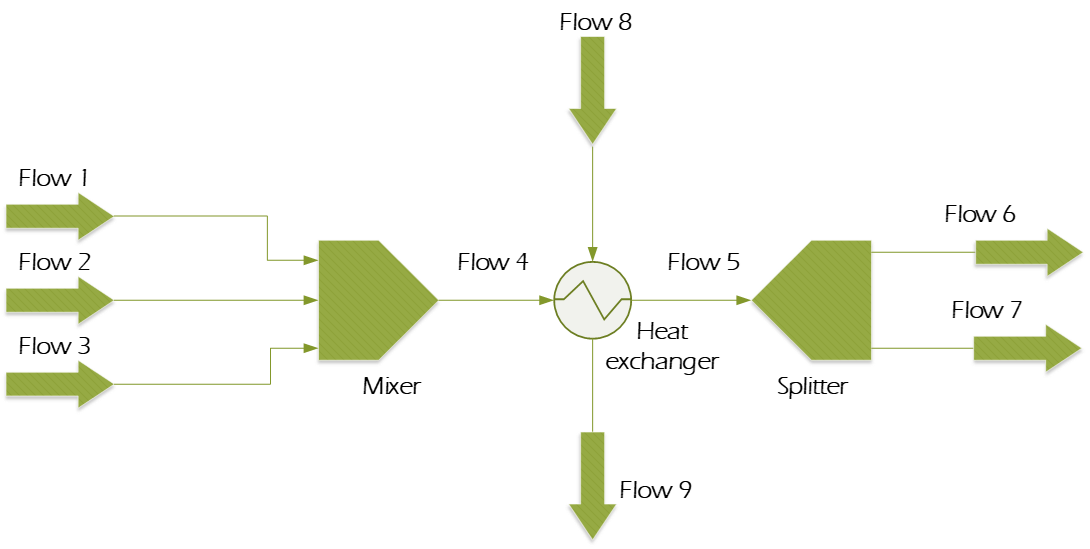
\includegraphics[width=.8\textwidth]{./pics/pfd}
\end{figure}
\vfill
Для решения поставленной задачи будет реализована объектная модель: каждый элемент химико-технологической системы будет описан как отдельный класс.
\vfill
\end{frame}

\subsection{Описание класса \texttt{Flow}}
\begin{frame}[fragile]{Описание класса \texttt{Flow}}
\scriptsize
\begin{table}[h!]
	\centering
	\renewcommand{\arraystretch}{1.2}
	\begin{tabular}{|p{.49\linewidth}|p{.49\linewidth}|}
		\hline
		\textbf{Атрибуты класса} & \textbf{Описание}  \\
		\hline
		\mintinline{python}|mass_flow_rate: float| & Массовый расход, кг / ч \\
		\hline
		\mintinline{python}|mole_flow_rate: float| & Мольный расход, кмоль / ч \\
		\hline
		\mintinline{python}|volume_flow_rate: float| & Объемный расход, м$^3$ / ч \\
		\hline
		\mintinline{python}|mass_fractions: np.ndarray| & Массовые доли \\
		\hline
		\mintinline{python}|mole_fractions: np.ndarray| & Мольные доли \\
		\hline
		\mintinline{python}|volume_fractions: np.ndarray| & Объемные доли \\
		\hline
		\mintinline{python}|temperature: float| & Температура потока, К \\
		\hline
		\mintinline{python}|density: float| & Плотность потока, г / см$^3$ \\
		\hline
		\mintinline{python}|average_mol_mass: float| & Средняя молекулярная масса потока, г / моль \\
		\hline
		\mintinline{python}|cp: float| & Массовая теплоемкость потока, кДж / кг \\
		\hline
\begin{minipage}{\linewidth}
\begin{minted}[frame=none, linenos=false]{python}
def __init__(
    self,
    mass_flow_rate: float,
    mass_fractions: np.ndarray,
    temperature: float
) -> None
\end{minted}
\end{minipage}
		& Создает новый экземпляр класса \texttt{Flow}, заполняя все поля \\
		\hline
	\end{tabular}
\end{table}
\vfill
\end{frame}

\subsection{Функции для пересчета составов}
\begin{frame}[fragile]{Функции для пересчета составов}
\scriptsize
\begin{enumerate}
\item Пересчет массовых долей в объемные:
\vfill
\begin{equation*}
	\varphi _i = \dfrac{\dfrac{\omega _i}{\rho _i}}{\sum \limits _{i=1}^{n} \dfrac{\omega _i}{\rho _i}}
\end{equation*}
\vfill
где $\varphi _i$~-- объемная доля $i$-го компонента; $\omega _i$~-- массовая доля $i$-го компонента; $\rho _i$~-- плотность $i$-го компонента; $n$~-- число компонентов в системе; $i$~-- индекс компонента в системе.
\vfill
\item Пересчет массовых долей в мольные:
\vfill
$$
	\chi _i = \dfrac{\dfrac{\omega _i}{M_i}}{\sum \limits_{i=1}^{n}\dfrac{\omega _i}{M_i}}
$$
\vfill
где $\chi _i$~-- мольная доля $i$-го компонента; $\omega _i$~-- массовая доля $i$-го компонента; $M_i$~-- молярная масса $i$-го компонента; $n$~-- число компонентов в системе; $i$~-- индекс компонента в системе.
\vfill
\end{enumerate}
\vfill
\end{frame}


\subsection{Функции для расчета плотности  и средней \\ молекулярной массы}
\begin{frame}[fragile]{Функции для расчета плотности и средней \\ молекулярной массы}
\scriptsize
\begin{enumerate}
\item Расчет плотности:
\vfill
\begin{equation*}
	\rho = \dfrac{1}{\sum \limits_{i=1}^{n}\dfrac{\omega_i}{\rho_i}}
\end{equation*}
\vfill
где $\rho$~-- плотность потока; $\omega _i$~-- массовая доля $i$-го компонента; $\rho _i$~-- плотность $i$-го компонента; $n$~-- число компонентов в системе; $i$~-- индекс компонента в системе.
\vfill
\item Расчет средней молекулярной массы потока:
\vfill
$$
	m = \dfrac{1}{\sum \limits_{i=1}^{n}\dfrac{\omega_i}{M_i}}
$$
\vfill
где $m$~-- средняя молекулярная масса потока; $\omega _i$~-- массовая доля $i$-го компонента; $M_i$~-- молярная масса $i$-го компонента; $n$~-- число компонентов в системе; $i$~-- индекс компонента в системе.
\vfill
\end{enumerate}
\vfill
\end{frame}

\subsection{Функции для расчета теплоемкости потока}
\begin{frame}[fragile]{Функции для расчета теплоемкости потока}
\scriptsize
Расчет теплоемкости потока в зависимости от состава потока и температуры среды осуществляется следующим образом:
\begin{itemize}
\item определяется теплоемкость компонентов потока при температуре среды:
\vfill
$$
	Cp_i = \sum \limits _{j=1} ^{5} j \cdot k\left[i, j\right] \cdot T^{j-1}
$$
\vfill
где $Cp_i$~-- теплоемкость $i$-го компонента, кДж / кг; $k\left[i, j\right]$~-- коэффициенты аппроксимации температурной зависимости энтальпии для $i$-го компонента; $T$~-- температура потока, К;
\vfill
\item определяется общая теплоемкость потока:
\vfill
$$
	Cp = \sum \limits _{i=1} ^{n} \omega _i \cdot Cp_i
$$
\vfill
где $\omega _i$~-- массовая доля $i$-го компонента; $Cp_i$~-- теплоемкость $i$-го компонента, кДж / кг; $n$~-- число компонентов в системе.
\end{itemize}
\vfill
\end{frame}

\section{Численное интегрирование}
\begin{frame}[fragile]{Численное интегрирование}
\scriptsize
Вычислим интеграл:
$$
I = \int\limits_{0}^{1}\dfrac{dx}{1 + x^2}
$$
при помощи функции \texttt{scipy.integrate.quad}.
\vfill
    \begin{tcolorbox}[breakable, size=fbox, boxrule=1pt, pad at break*=1mm,colback=cellbackground, colframe=cellborder]
\prompt{In}{incolor}{1}{\boxspacing}
\begin{Verbatim}[commandchars=\\\{\}]
\PY{k+kn}{from} \PY{n+nn}{scipy}\PY{n+nn}{.}\PY{n+nn}{integrate} \PY{k+kn}{import} \PY{n}{quad}
\end{Verbatim}
\end{tcolorbox}

    \begin{tcolorbox}[breakable, size=fbox, boxrule=1pt, pad at break*=1mm,colback=cellbackground, colframe=cellborder]
\prompt{In}{incolor}{2}{\boxspacing}
\begin{Verbatim}[commandchars=\\\{\}]
\PY{k}{def} \PY{n+nf}{func}\PY{p}{(}\PY{n}{x}\PY{p}{)}\PY{p}{:}
    \PY{k}{return} \PY{l+m+mi}{1} \PY{o}{/} \PY{p}{(}\PY{l+m+mi}{1} \PY{o}{+} \PY{n}{x} \PY{o}{*}\PY{o}{*} \PY{l+m+mi}{2}\PY{p}{)}
\end{Verbatim}
\end{tcolorbox}

    \begin{tcolorbox}[breakable, size=fbox, boxrule=1pt, pad at break*=1mm,colback=cellbackground, colframe=cellborder]
\prompt{In}{incolor}{3}{\boxspacing}
\begin{Verbatim}[commandchars=\\\{\}]
\PY{n}{a}\PY{p}{,} \PY{n}{b} \PY{o}{=} \PY{l+m+mi}{0}\PY{p}{,} \PY{l+m+mi}{1}
\PY{n}{res} \PY{o}{=} \PY{n}{quad}\PY{p}{(}\PY{n}{func}\PY{p}{,} \PY{n}{a}\PY{p}{,} \PY{n}{b}\PY{p}{)}
\PY{n}{res}
\end{Verbatim}
\end{tcolorbox}

            \begin{tcolorbox}[breakable, size=fbox, boxrule=.5pt, pad at break*=1mm, opacityfill=0]
\prompt{Out}{outcolor}{3}{\boxspacing}
\begin{Verbatim}[commandchars=\\\{\}]
(0.7853981633974484, 8.719671245021581e-15)
\end{Verbatim}
\end{tcolorbox}
\vfill
\end{frame}

\begin{frame}[fragile]{Численное интегрирование}
\scriptsize
\begin{itemize}
\item В тех случаях, когда подынтегральная функция принимает один или несколько параметров помимо своего основного аргумента, эти дополнительные параметры могут быть переданы в метод \texttt{quad} в виде кортежа в аргументе \texttt{args}.
Например, определим следующий интеграл в численном выражении:
	$$ I_{n,m} = \int\limits_{-\pi/2}^{\pi/2}\sin^nx\cos^mx\, dx $$
\end{itemize}
\vfill
    \begin{tcolorbox}[breakable, size=fbox, boxrule=1pt, pad at break*=1mm,colback=cellbackground, colframe=cellborder]
\prompt{In}{incolor}{4}{\boxspacing}
\begin{Verbatim}[commandchars=\\\{\}]
\PY{k+kn}{import} \PY{n+nn}{numpy} \PY{k}{as} \PY{n+nn}{np}
\end{Verbatim}
\end{tcolorbox}

    \begin{tcolorbox}[breakable, size=fbox, boxrule=1pt, pad at break*=1mm,colback=cellbackground, colframe=cellborder]
\prompt{In}{incolor}{5}{\boxspacing}
\begin{Verbatim}[commandchars=\\\{\}]
\PY{k}{def} \PY{n+nf}{func}\PY{p}{(}\PY{n}{x}\PY{p}{,} \PY{n}{n}\PY{p}{,} \PY{n}{m}\PY{p}{)}\PY{p}{:}
    \PY{k}{return} \PY{n}{np}\PY{o}{.}\PY{n}{sin}\PY{p}{(}\PY{n}{x}\PY{p}{)} \PY{o}{*}\PY{o}{*} \PY{n}{n} \PY{o}{*} \PY{n}{np}\PY{o}{.}\PY{n}{cos}\PY{p}{(}\PY{n}{x}\PY{p}{)} \PY{o}{*}\PY{o}{*} \PY{n}{m}
\end{Verbatim}
\end{tcolorbox}

    \begin{tcolorbox}[breakable, size=fbox, boxrule=1pt, pad at break*=1mm,colback=cellbackground, colframe=cellborder]
\prompt{In}{incolor}{6}{\boxspacing}
\begin{Verbatim}[commandchars=\\\{\}]
\PY{n}{n}\PY{p}{,} \PY{n}{m} \PY{o}{=} \PY{l+m+mi}{2}\PY{p}{,} \PY{l+m+mi}{3}
\PY{n}{quad}\PY{p}{(}\PY{n}{func}\PY{p}{,} \PY{o}{\PYZhy{}}\PY{n}{np}\PY{o}{.}\PY{n}{pi}\PY{o}{/}\PY{l+m+mi}{2}\PY{p}{,} \PY{n}{np}\PY{o}{.}\PY{n}{pi}\PY{o}{/}\PY{l+m+mi}{2}\PY{p}{,} \PY{n}{args}\PY{o}{=}\PY{p}{(}\PY{n}{n}\PY{p}{,} \PY{n}{m}\PY{p}{)}\PY{p}{)}
\end{Verbatim}
\end{tcolorbox}

            \begin{tcolorbox}[breakable, size=fbox, boxrule=.5pt, pad at break*=1mm, opacityfill=0]
\prompt{Out}{outcolor}{6}{\boxspacing}
\begin{Verbatim}[commandchars=\\\{\}]
(0.26666666666666666, 2.960594732333751e-15)
\end{Verbatim}
\end{tcolorbox}
\vfill
\end{frame}

\section{Системы ОДУ первого порядка}
\begin{frame}[fragile]{Система взаимосвязанных ОДУ первого порядка}
\scriptsize
Рассмотрим следующую схему химических реакций:

$$A \rightarrow B \rightarrow C$$

\noindent с константами скоростей $k_1$ и $k_2$. Уравнения, описывающие скорость изменения концентраций компонентов по времени, записываются следующим образом:

\begin{equation*}
	\left\{
	\begin{aligned}
		\dfrac{d\left[A\right]}{dt} &= -k_1\left[A\right] \\
		\dfrac{d\left[B\right]}{dt} &=  k_1\left[A\right] - k_2\left[B\right] \\
		\dfrac{d\left[C\right]}{dt} &=  k_2\left[B\right] \\
	\end{aligned}
	\right.
\end{equation*}


Для численного решения предположим $y_1 \equiv \left[A\right]$,  $y_2 \equiv \left[B\right]$ и $y_3 \equiv \left[C\right]$:
\begin{equation*}
	\left\{
	\begin{aligned}
		\dfrac{d\left[A\right]}{dt} &= -k_1y_1 \\
		\dfrac{d\left[B\right]}{dt} &=  k_1y_1 - k_2y_2 \\
		\dfrac{d\left[C\right]}{dt} &=  k_2y_2 \\
	\end{aligned}
	\right.
\end{equation*}
\vfill
\end{frame}

\begin{frame}[fragile]{Система взаимосвязанных ОДУ первого порядка}
\scriptsize
Зададимся значениями констант: $k_1 = 0.2 \text{ } c^{-1}$, $k_2 = 0.8 \text{ } c^{-1}$ и начальными условиями: $y_1(0) = 100$, $y_2(0) = 0$ $y_3(0) = 0$.
\vfill
    \begin{tcolorbox}[breakable, size=fbox, boxrule=1pt, pad at break*=1mm,colback=cellbackground, colframe=cellborder]
\prompt{In}{incolor}{1}{\boxspacing}
\begin{Verbatim}[commandchars=\\\{\}]
\PY{k+kn}{import} \PY{n+nn}{numpy} \PY{k}{as} \PY{n+nn}{np}
\PY{k+kn}{from} \PY{n+nn}{scipy}\PY{n+nn}{.}\PY{n+nn}{integrate} \PY{k+kn}{import} \PY{n}{solve\PYZus{}ivp}
\end{Verbatim}
\end{tcolorbox}

    \begin{tcolorbox}[breakable, size=fbox, boxrule=1pt, pad at break*=1mm,colback=cellbackground, colframe=cellborder]
\prompt{In}{incolor}{2}{\boxspacing}
\begin{Verbatim}[commandchars=\\\{\}]
\PY{n}{k1}\PY{p}{,} \PY{n}{k2} \PY{o}{=} \PY{l+m+mf}{.2}\PY{p}{,} \PY{l+m+mf}{.8}
\PY{n}{y0} \PY{o}{=} \PY{l+m+mi}{100}\PY{p}{,} \PY{l+m+mi}{0}\PY{p}{,} \PY{l+m+mi}{0}
\PY{n}{t0}\PY{p}{,} \PY{n}{tf} \PY{o}{=} \PY{l+m+mi}{0}\PY{p}{,} \PY{l+m+mi}{20}
\end{Verbatim}
\end{tcolorbox}

    \begin{tcolorbox}[breakable, size=fbox, boxrule=1pt, pad at break*=1mm,colback=cellbackground, colframe=cellborder]
\prompt{In}{incolor}{3}{\boxspacing}
\begin{Verbatim}[commandchars=\\\{\}]
\PY{k}{def} \PY{n+nf}{func}\PY{p}{(}\PY{n}{t}\PY{p}{,} \PY{n}{y}\PY{p}{,} \PY{n}{k1}\PY{p}{,} \PY{n}{k2}\PY{p}{)}\PY{p}{:}
    \PY{n}{y1}\PY{p}{,} \PY{n}{y2}\PY{p}{,} \PY{n}{y3} \PY{o}{=} \PY{n}{y}
    \PY{n}{dy1dt} \PY{o}{=} \PY{o}{\PYZhy{}}\PY{n}{k1} \PY{o}{*} \PY{n}{y1}
    \PY{n}{dy2dt} \PY{o}{=} \PY{n}{k1} \PY{o}{*} \PY{n}{y1} \PY{o}{\PYZhy{}} \PY{n}{k2} \PY{o}{*} \PY{n}{y2}
    \PY{n}{dy3dt} \PY{o}{=} \PY{n}{k2} \PY{o}{*} \PY{n}{y2}

    \PY{k}{return} \PY{n}{dy1dt}\PY{p}{,} \PY{n}{dy2dt}\PY{p}{,} \PY{n}{dy3dt}
\end{Verbatim}
\end{tcolorbox}
\vfill
\end{frame}

\begin{frame}[fragile]{Система взаимосвязанных ОДУ первого порядка}
\scriptsize
    \begin{tcolorbox}[breakable, size=fbox, boxrule=1pt, pad at break*=1mm,colback=cellbackground, colframe=cellborder]
\prompt{In}{incolor}{4}{\boxspacing}
\begin{Verbatim}[commandchars=\\\{\}]
\PY{n}{solution} \PY{o}{=} \PY{n}{solve\PYZus{}ivp}\PY{p}{(}
    \PY{n}{func}\PY{p}{,} \PY{p}{(}\PY{n}{t0}\PY{p}{,} \PY{n}{tf}\PY{p}{)}\PY{p}{,} \PY{n}{y0}\PY{p}{,} \PY{n}{dense\PYZus{}output}\PY{o}{=}\PY{k+kc}{True}\PY{p}{,}
    \PY{n}{args}\PY{o}{=}\PY{p}{(}\PY{n}{k1}\PY{p}{,} \PY{n}{k2}\PY{p}{)}
\PY{p}{)}
\PY{n}{t} \PY{o}{=} \PY{n}{np}\PY{o}{.}\PY{n}{linspace}\PY{p}{(}\PY{n}{t0}\PY{p}{,} \PY{n}{tf}\PY{p}{,} \PY{l+m+mi}{10}\PY{p}{)}
\PY{n}{a}\PY{p}{,} \PY{n}{b}\PY{p}{,} \PY{n}{c} \PY{o}{=} \PY{n}{solution}\PY{o}{.}\PY{n}{sol}\PY{p}{(}\PY{n}{t}\PY{p}{)}
\end{Verbatim}
\end{tcolorbox}

    \begin{tcolorbox}[breakable, size=fbox, boxrule=1pt, pad at break*=1mm,colback=cellbackground, colframe=cellborder]
\prompt{In}{incolor}{5}{\boxspacing}
\begin{Verbatim}[commandchars=\\\{\}]
\PY{k}{for} \PY{n}{ai}\PY{p}{,} \PY{n}{bi}\PY{p}{,} \PY{n}{ci} \PY{o+ow}{in} \PY{n+nb}{zip}\PY{p}{(}\PY{n}{a}\PY{p}{,} \PY{n}{b}\PY{p}{,} \PY{n}{c}\PY{p}{)}\PY{p}{:}
    \PY{n+nb}{print}\PY{p}{(}\PY{l+s+sa}{f}\PY{l+s+s1}{\PYZsq{}}\PY{l+s+si}{\PYZob{}}\PY{n}{ai}\PY{l+s+si}{:}\PY{l+s+s1}{\PYZgt{}8.2f}\PY{l+s+si}{\PYZcb{}}\PY{l+s+s1}{ }\PY{l+s+si}{\PYZob{}}\PY{n}{bi}\PY{l+s+si}{:}\PY{l+s+s1}{\PYZgt{}8.2f}\PY{l+s+si}{\PYZcb{}}\PY{l+s+s1}{ }\PY{l+s+si}{\PYZob{}}\PY{n}{ci}\PY{l+s+si}{:}\PY{l+s+s1}{\PYZgt{}8.2f}\PY{l+s+si}{\PYZcb{}}\PY{l+s+s1}{\PYZsq{}}\PY{p}{)}
\end{Verbatim}
\end{tcolorbox}

    \begin{Verbatim}[commandchars=\\\{\}]
  100.00     0.00     0.00
   64.12    15.74    20.14
   41.11    12.75    46.14
   26.36     8.63    65.02
   16.90     5.61    77.49
   10.84     3.61    85.56
    6.95     2.31    90.74
    4.45     1.49    94.06
    2.86     0.95    96.19
    1.83     0.61    97.56
    \end{Verbatim}
\vfill
\end{frame}

\section{Задания}
\sectionframe

\begin{frame}[fragile]{\textcolor{tpugreen}{\textbf{Задание~1}}}
\scriptsize
Дана зависимость энтальпии от температуры:
\vfill
\begin{table}
%	\caption{Этилбензол $C_8H_{10}$}
\begin{tabular}{|c|c|}
	\hline
	T, K & $\Delta H$, кДж/моль \\
	\hline
	300 & 29.62  \\
	\hline
	400 	& 21.88 \\
	\hline
	500    & 15.52 \\
	\hline
	600  & 10.38 \\
	\hline
	700  & 6.40 \\
	\hline
	800  & 3.35 \\
	\hline
	900  & 1.13 \\
	\hline
	1000  & 0.21 \\
	\hline
\end{tabular}
\end{table}
\vfill
Определить значения энтальпии при изменении $Т$ от $300$ до $1000$ с шагом $50$ К, используя:
\begin{enumerate}
	\item Кубический сплайн;
	\item Линейную аппроксимацию.
\end{enumerate}
\vfill
\end{frame}

\begin{frame}[fragile]{\textcolor{tpugreen}{\textbf{Задание~2}}}
\scriptsize
Используя функцию \texttt{scipy.integrate.quad}, вычислите значение энтропии воды при ее нагревании от $400$ до $500$~К по формуле:
	$$ \Delta S = \eta \cdot \int\limits_{400}^{500} \dfrac{C_v \cdot dT}{T} $$
Количество молей $\eta = 3$; значение теплоемкости $C_v = 35.0$ Дж / (моль $\cdot$ К).
\vfill
\end{frame}

\begin{frame}[fragile]{\textcolor{tpugreen}{\textbf{Задание~3}}}
\scriptsize
Дана схема химических превращений:
\begin{center}
\schemestart
	C \arrow{<->[$k_2$][$k_3$]}[30] A \arrow{->[$k_1$]}[-30] B
\schemestop

\begin{minipage}{.45\textwidth}
\begin{align*}
	C_{A_0} &= 0.7 \left(\text{моль/л}\right); &\quad k_1 &= 0.21 \left(c^{-1}\right); \\
	C_{B_0} &= 0.0 \left(\text{моль/л}\right); &\quad k_2 &= 0.12 \left(c^{-1}\right); \\
	C_{C_0} &= 0.0 \left(\text{моль/л}\right); &\quad k_3 &= 0.18 \left(c^{-1}\right).\\
\end{align*}
\vfil
\end{minipage}
\begin{minipage}{.5\textwidth}
\begin{equation*}
\left\{
	\begin{aligned}
		\dfrac{dC_A}{dt} &= -k_1 \cdot C_A -k_2 \cdot C_A + k_3 \cdot C_C \\
		\dfrac{dC_B}{dt} &=  k_1 \cdot C_A  \\
		\dfrac{dC_C}{dt} &=  k_2 \cdot C_A - k_3 \cdot C_C \\
	\end{aligned}
\right.
\end{equation*}
\end{minipage}
\end{center}


\vfill
\end{frame}

\contactsframe[\Large \textbf{Благодарю за внимание!}]{

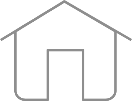
\includegraphics[width=.05\textwidth]{pics/home} \quad Учебный корпус №2, ауд. 136 \\

\includegraphics[width=.05\textwidth]{pics/mail} \quad chuva@tpu.ru \\

\includegraphics[width=.03\textwidth]{pics/tel} \quad +7-962-782-66-15
}

\end{document}

